\documentclass{article}
\usepackage[margin=.9in]{geometry}
\usepackage{xcolor}
\usepackage{amsmath}
\usepackage{amssymb}
\usepackage{float}
\usepackage{listings}
\lstset{
  basicstyle=\small\ttfamily,
  breaklines=true,
  frame=single,
  language=Verilog,
  numberstyle=\tiny,
  showstringspaces=false
}
\setlength{\parindent}{0pt}
\setlength{\parskip}{\baselineskip}
\definecolor{mycolor}{rgb}{0.1, 0.1, 0.5}
\title{\textbf{{\huge Voltage Controlled Oscillator Design}}}
\author{Christopher Hunt}
\date{}
\usepackage{graphicx} 
\usepackage{fancyhdr}

\begin{document}
\pagestyle{fancy}
\fancyhf{}
\rfoot{ENGR 203}
\lfoot{Christopher HUnt}
\lhead{VCO Design}
\rhead{\thepage}
\maketitle
\section*{\textcolor{mycolor}{Abstract}}
The aim of this lab is to design and analyze a simple sawtooth oscillator based on an inverting Schmitt trigger circuit. The oscillator's frequency is controlled by a voltage input, which modulates the behavior of an NPN transistor. We will investigate the signals that control the NPN transistor and study its response characteristics. The project will involve building the oscillator circuit, implementing signal analysis techniques, and exploring the effects of different control voltages on the oscillator's output waveform.

To accomplish the objectives of this lab project, we will first construct the sawtooth oscillator circuit using an inverting Schmitt trigger and NPN transistor. We will then examine the behavior of the NPN transistor by studying the signals that control its openness. Additionally, operational amplifiers and AC coupling will be used to eliminate DC offset and enhance the quality of the output waveform.

Through this project, we will gain insights into voltage-controlled oscillators, NPN transistor behavior, and the impact of control signals on the oscillator's output.
\vspace{5mm}
\hrule

\section*{\textcolor{mycolor}{Equipment}}
\begin{itemize}
  \item Siglent SDS 1202X-E Serial: SDS1EDEQ6R7384
  \item HP 6236B Triple Output Power Supply Serial: 15175
  \item AstroAI DM6000AR Multimeter
  \item Korg SQ-1 Serial: 048860
\end{itemize}
\vspace{5mm}
\hrule

\section*{\textcolor{mycolor}{Design}}
A Voltage Controlled Oscillator (VCO) is an electronic circuit that utilizes an input voltage to regulate and modify the frequency of the generated oscillating waveform. In this lab, the VCO design centers around an inverting Schmitt Trigger, which incorporates hysteresis with two distinct trigger points: a higher threshold voltage ($V_{High}$) and a lower threshold voltage ($V_{Low}$).

In this specific design, an inverting Schmitt Trigger is carefully selected to achieve the desired functionality. When the circuit is powered, the Schmitt Trigger initially produces a high signal. Once the input voltage surpasses the $V_{High}$ threshold, the output switches to a low signal. Conversely, when the input voltage drops below the $V_{Low}$ threshold, the output switches back to a high signal. This behavior is achieved by employing a diode to feed the trigger's output back to its input.

To introduce the voltage-controlled behavior of the oscillator, a capacitor is connected to the same input node as the Schmitt Trigger. Upon powering the circuit, the capacitor starts to charge. As soon as the voltage on the capacitor reaches the $V_{High}$ threshold, the Schmitt Trigger turns off, causing the capacitor to discharge. This discharge process extends the duration during which the input voltage remains above the $V_{Low}$ threshold.

The rate at which the capacitor discharges can be precisely controlled by adjusting the resistance between the input node and ground. Placing a potentiometer at this point enables manual adjustment of the oscillator's frequency. Alternatively, this adjustment can be automated using transistors. By replacing the potentiometer with an NPN transistor between the input and ground, the amount of current passing from the input node to ground can be modulated by varying the voltage at the transistor's base.

For this specific design, a combination of NPN and PNP transistors is employed, with the PNP transistor configured as an emitter follower. This arrangement effectively addresses potential temperature effects that might challenge a single transistor in maintaining a constant current, potentially impacting the frequency of the sawtooth wave. The NPN and PNP transistors essentially operate in an inverse manner with respect to temperature. As the temperature rises, the NPN transistor opens up, allowing more current to flow. Conversely, the PNP transistor starts to restrict current flow, raising the voltage at the base of the NPN transistor. This process counteracts the temperature's influence, resulting in more stable capacitor drainage and, consequently, a more consistent output frequency.

To facilitate voltage control, the base of the PNP transistor serves as the control point. A simulated potentiometer, achieved by a voltage divider between $V_{pos}$ and $V_{neg}$, allows for setting the lowest frequency when the control voltage is at zero. The external voltage signals applied at $VC$ can then modify the frequency by modulating the voltage applied to the base, providing the VCO with versatile control options.

Subsequently, the generated sawtooth wave is directed to the positive terminal of an amplifier circuit. This circuit plays a crucial role in decoupling the generator from the output, removing any DC offset using AC coupling, and amplifying the output to an appropriate voltage range for subsequent signal processing.

By implementing these components and configurations, the VCO design achieves precise voltage-controlled frequency modulation and incorporates measures to compensate for temperature effects, ensuring stable performance and facilitating signal processing in further stages.


\begin{figure}[H]
  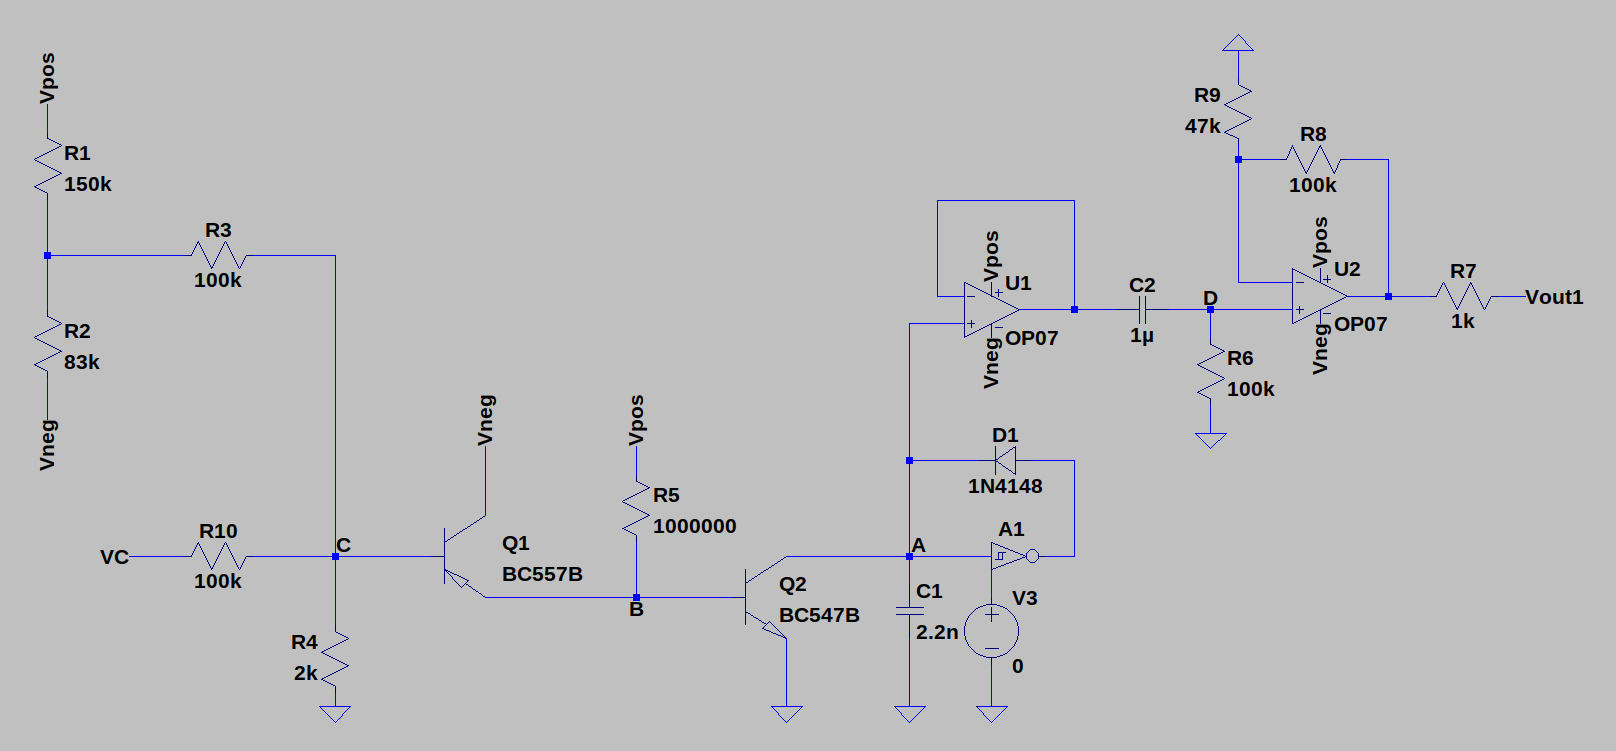
\includegraphics[width=1\linewidth]{vco_schem.png}
  \caption{VCO Schematic}
\end{figure}


\section*{\textcolor{mycolor}{Simulation}}
\vspace{5mm}
\hrule


\section*{\textcolor{mycolor}{Implementation}}
\vspace{5mm}
\hrule

\section*{\textcolor{mycolor}{Conclusion}}
Summary of the lab and its outcomes
\vspace{5mm}
\hrule

\end{document}